Scopo di questo capitolo è fare un'introduzione sulle tecniche da vuoto. Tale argomento è di nostro interesse perché si ritrova in tanti campi applicativi.

Parleremo sia di come si produce il vuoto che di come si misura.

\section{Una breve introduzione}

\subsection{Un po' di storia}
Facciamo innanzitutto un'introduzione generale sul sul vuoto.

Il concetto di vuoto nasce in filosofia, dove fu introdotto per la prima volta da democrito con la sua teoria atomista della materia. Per tanto tempo tale concetto non fu accettato, tant'è che si parlava di horror vacui, cioè la paura del vuoto, un teoria ideata da Aristotele e ritenuta valida fino ai tempi di Cartesio che respingeva questo concetto secondo cui potesse esistere una regione priva di materia. Più tardi, Galileo studiò il vuoto sperimentalmente attraverso una pompa aspirante abbastanza rudimentale. Nel 1644 viene costruito il primo barometro\footnote{Il barometro voi è un misuratore di pressione, in particolare di pressioni prossime al valore della pressione atmosferica.} a mercurio ad opera di Torricelli. La prima pompa da vuoto venne utilizzata nel 1654 per la dimostrazione delle sfere di Magdeburgo.

Il primo vacuometro (cioè un misuratore di pressione per pressioni che sono molto al di sotto della pressione atmosferica) venne realizzato nel 1850 da McLeod, mentre la prima pompa rotativa, che è una tipologia di pompa che adopereremo in laboratorio, risale al 1905.

\subsection{Unità di misura}
Dal punto di vista fisico in generale si utilizza la parola vuoto con due accezioni:
\begin{itemize}[leftmargin=0.5cm]
   \item o per indicare uno spazio totalmente privo di materia;
   \item oppure, in maniera più corretta, per indicare una regione di spazio che è occupata da aeriformi con una pressione che risulta essere più bassa rispetto a quella atmosferica.
\end{itemize}
Nel sistema internazionale la pressione si misura in Pascal (Pa), cioè in $\rm N/m^2$, ma esistono tante altre unità di misura per indicare la pressione le quali vengono adoperate in contesti differenti, ad esempio spesso quando si fa riferimento alle condizioni meteorologiche si usa il millibar.

Solitamente il nostro riferimento è la pressione atmosferica, dunque diamo qualche indicazione su questa quantità.

La pressione atmosferica ovviamente è definita attraverso il rapporto tra il peso esercitato da una colonna d'aria e l'unità di superficie. Il suo valore varia in funzione dell'altezza.
\begin{figure}[H]
   \centering
   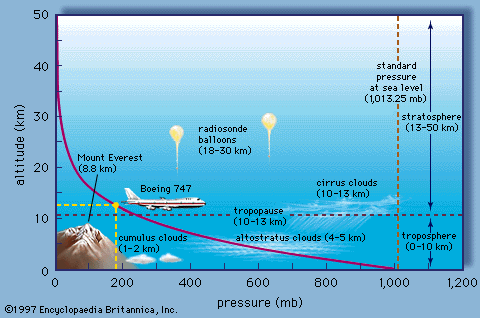
\includegraphics[width=0.7\textwidth]{immagini/pressione_atmosferica.png}
\end{figure}
Nella figura sopra possiamo vedere il valore della pressione atmosferica al variare dell'altitudine, riportata in chilometri. Al livello del mare abbiamo valori tipici di pressione tra i 900 e i 1000 mbar a cui siamo abituati, ma man mano che aumenta l'altitudine la pressione diminuisce parecchio ad esempio in corrispondenza del Monte Everest, cioè a un'altitudine di quasi 9 km, la pressione atmosferica diventa pari a 250 mbar, quindi si è ridotta a un quarto del valore sul livello del mare.

\textbf{continua a 1:36:38 circa}

La pressione atmosferica non è costante, lo sapete, ha delle variazioni, magari lo sapete in termini di variazioni grosso l'anee cioè delle decine di mili bar che sono le variazioni legate alle variazioni del medio quindi quando parliamo di periodi di bassa pressione alta pressione sono collegata appunto a periodi di brutto tempo, bell tempo allora li parliamo di variazioni consistenti della pressione atmosferica di decine di mili bar. Ma in realtà questa pressione varia anche periodicamente in intervalli più piccoli delle 24 ore. Vedete ad esempio esempio in questo grafico l'andamento della pressione misurata con sensore di pressione qui a livello di il mare in funzione del tempo in un arco temporale di 300 ore. Oltre a variazioni impreudisi come vedete qui che siamo passati da 1.700 a 997 a 998 mili bar questo è chiaramente un periodo di bassa pressione quindi del fatto che il tempo stava peggiorando ma oltre a questo se vedete sovrapposto ci sono delle piccole oscillazioni che sono appunto dell'ordine delle 24 ore perché sono le variazioni sostanzialmente giorno notte quindi legate anche alla temperatura sono le condizioni generali della nostra atmosfera che cambiano giornalmente e sono variazioni ovviamente più piccole che sono più difficili per rivelare di pochi mili bar quindi quando noi parliamo di pressione atmosferica è vero noi facciamo riferimento a un valore generico ma in realtà dobbiamo sempre tener conto del fatto che questo valore cambia con l'altitudine e cambia anche nel corso del tempo e questo per conto riguarda ciò che avviene sulla terra ma se noi ci spostiamo fuori dall'atmosfera terrestre andiamo incontro ad altri altri valori di pressione qui stiamo parlando sempre di pressione diciamo naturale quindi di vuoto naturale ad esempio se andassimo sulla superficie lunare ci renderemo conto che innanzitutto sono presenti in gas come idrogeno, elione o neargon ma a pressioni estremamente basse parliamo di 10 a la man 8 mili bar da confrontare con all'incirca i 10 alla 3 mili bar della nostra pressione atmosferica a livello del mare quindi vedete siamo ben 11 ordini di grandezza più sotto rispetto a quello che viene sulla terra è proprio per questo motivo in questi contesti piuttosto che utilizzare questa unità di misura si preferisce blondare a un altro riferimento cioè parlare in termini di numero di atomi o molecole per centimetro cubo o metro cubo, diventa più facile a quel punto e giusto per avere un'idea vedete qui alcuni uoti caratteristici dell'universo. Ad esempio, se ci spossiamo dalla terra a una distanza di mille chilometri, ci ritroviamo 5 per 10 alla 5 particelle per centimetro cubo, che sono veramente poche, ma se andiamo in altri quantessi, praticamente abbiamo una riduzione drastica, ad esempio nelle nuove, l'interstellare parliamo solamente di 8 particelle per centimetro cubo e in generale prendere in considerazione tutto l'universo, quindi l'essenzione dell'universo e le cose da cui è composto, si parla di impressioni dell'ordine di 1 per 10 alla menzette particelle su centimetro cubo. Quindi capite che questi sono ovviamente condizioni estreme verso cui noi non potremmo mai andare con delle attrezzature sperimentale, quindi quindi ovviamente dei vuoti limite. Ora andremo a vedere invece che cosa si può realizzare attraverso afferettature. Prima di parlare proprio dei sistemi da vuoto, voglio dirvi accennarvi ad alcune applicazioni del vuoto, proprio per farvi capire che effettivamente la tecnologia del vuoto non solo ha avuto dei miglioramenti notevoli nel corso degli anni, ma in più trova applicazioni in svariati contesti. Allora innanzitutto la tecnologia del vuoto ha permesso in fisica di effettuare tantissime scoperte, pensiamo ad esempio, banalmente, all'effetto fotoelettrico che è stato studiato appunto all'interno di una valva di un bulbo dove viene realizzata il vuoto, oppure permette di sviluppare nuove tecniche di analisi, ad esempio la tecnica di spettroscopia di massa, non so se avete fatto in fisico di sfrutturare, o qualcuno dice di sì, solo una ragazza dice di sì, non so gli altri davvero, no questo è il il Va bene, se lo ricordo, quindi è stato fatto, poi lo risunirete, prevede ovviamente l'utilizzo del vuoto, oppure è stato utilizzato per costruire dei macchinari di indagine, pensato ad esempio agli acceleratori di particelle che hanno permesso di capire la struttura della materia andando sempre più nel microscopico e facendo viaggiare dei fasci che necessariamente devono viaggiare in un ambiente presso che è vuoto. Oggi si raggiungono dei valori di pressione estremamente bassi, ad esempio si riesce ad arrivare a 10 a la mezz'iove millibar su volumi abbastanza stessi, abbastanza grandi, ad esempio come nel caso degli acceleratori, oppure vuoti ancora più spinti, 10 a la mezz'iove millibar, ad esempio nel campo della ricerca sui materiali, cioè tutti quei campi laddove magari si lavora con pochi strati di atomi e si vuole anche evitare magari contaminazioni superficiali, cioè di fatto che magari questo materiale si trova all'interno di un ambiente dove sono presenti mollicole di gas che possono chiaramente falsare le proprietà di questi materiali. L'impianto di alto vuoto più grande al mondo è costituito dagli interferometri per la rivelazione delle onde gravitazionali di cui avete sicuramente sentito parlare i anni passati, quindi in Italia e nell'usa. E vi dicevo il vuoto è indispensabile per 

tantissimi applicazioni, questo è una foto di questo interferometro in particolare quello di salato a cascina vicino a Pisa, è costituito, l'avrete visto certamente da due rami che poi si congiungono, la lunghezza sono mi sbaglio è di diversi chilometri, vi vi vi so modo, quindi immaginate di aver praticare il vuoto in tubi che comunque hanno una dimensione considerabile. C'è scritto 3 chilometri. E quindi andiamo a guardare un po' le le applicazioni e che il livello di vuoto si aggiunge. Il vuoto può essere utilizzato ad esempio nel caso di simulazioni spaziali, voglio vedere come funziona una vermiata parecchiatura nel vuoto. In questo caso vedete non sono vuoti particolarmente, comunque se possono aggiungere si anche vuoti particolarmente spinti oppure in preparazione di finzottili come vi ho detto prima o in metallurgia, la dove volete ad esempio realizzare delle fusioni e delle le di sotto vuoto magari con materiali particolarmente reattivi e quindi volete evitare che durante la fusione intervenga l'interazione con qualche molecolo gas o atomo di un gas negli acceleratori di particelle. Nella fisica dei plasmi, le macchine per la fusione nucleare, l'iofilizzazione, il solamento termico insomma ci sono tantissime applicazioni che possono essere sia di natura scientifica quindi nel campo della ricerca sia di natura tecnologica. Ad esempio se ci limitiamo nel campo scientifico qui sono riportati alcuni esempi ad esempio c'è la spettrometria di massa di cui si ricordo solo la vostra vollega ed è indicato di la zona regione di vuoto dove si opera e vedete ci sono diverse fasce in base alla pressione in generale ora lo vedremo la pressione si distingue ovviamente non è una distinzione proprio netta è un'indicazione in base al valore della pressione tra vuoto grosso lano, vuoto medio, alto vuoto e ultra vuoto, ultra alto vuoto. Vedete ad esempio per le spettrometri di massa ci troviamo già in una regione di alto vuoto. Se andiamo a vedervi acceleratori di particelle vedete che ci stiamo spingendo verso l'ultra alto vuoto e così via diversi campi in questo caso della ricerca. Questi sono alcuni esempi, già abbiamo detto acceleratori perché è necessario produrre vuoto in un acceleratore perché dobbiamo evitare che le particelle che compongono il fascio che sta circolando vado a interagire con gli atomi o le molecole del gas residuo perché altrimenti ovviamente perdiamo quella particella oppure esperimenti della materia condensata dove vi dicevo in generale si studiano superfici o pochi strati atomici della materia o ancora è importante simulare le situazioni fisiche che si verificano nello spazio planetario per andare a vedere a far delle prove su satellite, su navi spaziali o ancora controllare la pressione nel gas in esame in alcuni casi specifici di riduzione in tubi etronici o in altri sistemi in cui si studia la scarica nel gas. Del punto di vista tecnologico non è da meno l'importanza del vuoto e addirittura a certe volte si riede anche un vuoto ancora più spinto rispetto a quello che si utilizza nel campo della ricerca. Alcuni esempi potrebbero essere questi isolamento termico creando delle intercapedini in cui viene creato il vuoto. Spesso l'isolamento termico che si realizza anche negli edifici si realizza con intercapedini infatti di aria, ad esempio le camere doppiobetro delle finestre hanno proprio questa funzione, creare un isolamento termico e capite che appunto questo questo è spinto ancora di più utilizzando tecniche da vuoto. Chiaramente non lo si fa per l'abitazione casalinga ma si fa in determinati contesti come ad esempio questi contentoni dei liquidi freddi, i DuWars. Oppure si può utilizzare per rallentare i processi di decomposizione organica dovuta agli agenti aerobici, quindi quindi caso di materiale organico sotto vuoto. Altre cose, evitare scariche in gas, reazioni chimiche su un filamento o eliminare gas di sciolte in un dato materiale, il processo di liofilizzazione. Ci sono anche tantissime applicazioni al punto di vista tecnologico che rendono il vuoto un aspetto perche importante. Allora andiamo a vedere la distinzione, i diversi livelli di vuoto che abbiamo visto in precedenza in maniera molto veloce. Ora qui lo stiamo vedendo in questa tabella dove andiamo a distinguere il vuoto, quindi partendo dalla pressione atmosferica e arrivando all'ultra vuoto. Vediamo il valore di pressione corrispondente, il valore limite di pressione corrispondente a questi intervalli, la densità di particelle e il libero camminometrio valutato a una temperatura di 300 Kelvin. E vedete quindi che ci sono diversi ordini di grandezza, dal vuoto grossolano una millimetro di mercurio fino all'ultra vuoto. Parliamo di 13 ordini di grandezza che si possono esplorare. E allora come si realizza un vuoto? Come è fatto un sistema da vuoto? Abbiamo bisogno innanzitutto di un recipiente, quella che noi chiamiamo camera da vuoto, da cui noi vogliamo estrarre l'aria, se è aria o qualsiasi altro gas che è contenuto in esso. Questa camera da vuoto deve essere collegata attraverso un condotto a un sistema che aspira, quindi quella che noi chiamiamo pompa. Il condotto può provvedere eventualmente una valvola di apertura e di chiusura, che è quella che io ad esempio nella camera da vuoto delle alfa vi ho indicato, vi ho detto qui in base alla posizione che noi noi aprire o chiudere il collegamento con la pompa. Spesso è prevista anche una valvola di rientro dell'aria, cioè una valvola che è una volta aperta fa rientrare l'aria dall'esterno verso l'interno. Qui abbiamo bisogno di una camera, di un inchianto di pompaggio, qualcosa che va da misurare una strumentazione che va da misurare il livello di vuoto raggiunto, perché è importante saperlo, e chiaramente poi un insieme di giunti, valvole condotti, trappole, guarnizioni, che va a corredare tutto il sistema da vuoto, perché capite che ogni elemento che viene connesso deve essere curato dal punto di vista delle perdite, quindi la pompa che deve essere connessa al condotto che va verso la camera, chiaramente deve essere connessa con delle opportune guarnizioni da vuoto, degli o ring, quindi bisogna curare eventuali perdite del sistema. In generale i sistemi da vuoto si distinguono in sigillati, viene prodotta il vuoto fino a un certo livello e viene chiusa, sperando che non ci siano perdite, in maniera tale che questo vuoto si dovrebbe mantenere nel tempo, si parla di vuoto statico, oppure un pompaggio continuo, un vuoto dinamico, perché il sistema di pompaggio è continuamente in funzione e si crea ovviamente un equilibrio, perché si deve mantenere questo sistema in funzione, perché evidentemente il sistema da vuoto presenta delle perdite, quindi se io provo a realizzare un vuoto statico, dopo un certo tempo il rientro di aria all'interno della camera è tale che il vuoto si vederà da, quindi devo mantenere continuamente attiva il sistema di pompaggio in maniera tale da assicurare un certo livello di vuoto, ed è il nostro caso che per le vostre recchie non sarà per niente gradevole, velovitici, per le mie ovviamente, quindi avere questa pompa ratativa sempre attiva non è piacevole. Questo è il caso ideale, ma in realtà la camera da vuoto ha delle perdite, è impossibile realizzare

un sistema senza perdite e quindi ci potrebbero essere dei casi in cui sia l'introduzione di auto, mio molecole di gas all'interno della camera. Ora non necessariamente devono essere perdite, cioè aria che entra all'interno della camera potrebbe essere anche generato da altro, ad esempio vedremo che le pompe che spesso sono pompe che prevedono il movimento meccanico di parti meccaniche, devono essere lubrificate con degli oli, con degli hidrocarburi e spesso vapori di questi oli possono andare all'interno della camera e quindi creare una pressione resiglia inevitabila, ma vedete queste sono tutte le fonti possibili di rientro, quindi perdite del recipiente oppure vapori di varia natura o anche le pareti stesse della camera che magari rilascia del gas. Quindi purtroppo dobbiamo sempre tener conto del fatto che ci può essere questo aspetto negativo che richiede magari un pompaggio continuo. Allora nello studiare un sistema da vuoto, ora vedremo alcune leggi fondamentali, bisogna fare riferimento a queste due grandezze. Una è la portata volumetrica che si indica normalmente con sigma che è anche detta velocità di pompaggio, cioè rappresenta il volume di gas che viene aspirato dalla pompa dell'unità di tempo quindi si esprime in metri cubi al secondo. Guardando ad esempio quel condotto che collega la pompa alla camera rappresenta quanta area passa in quel condotto nell'unità di tempo. Scopriremo dell'anticico che in realtà noi ora qua siamo generalmente parlando di sigma, ma ci sarà una sigma di partenza della pompa quindi all'inizio del condotto e alla fine del condotto quindi in prossimità dell'ingresso della camera quindi qui ci sarà una sigma efficace cioè c'è una perdita purtroppo attraverso il condotto. Noi si parlerà di legge di ohm nel caso del vuoto quindi faremo un confronto con quello che avviene con una resistenza. Nella resistenza c'è una caduta di potenziale, qui abbiamo una caduta della portata quindi è una legge praticamente simile alla legge di ohm quindi in velo anticipo parliamo di portata volumetrica ma in realtà sarà qualcosa di un po' più complesso. Poi abbiamo la portata q che dipende, vedete è una grandezza che tiene conto anche della pressione da cui si parte quindi è il prodotto della pressione all'interno della camera per sigma. Quindi in unità di misure capite si misura in metri cubi per pascalo al secondo perché questa grandezza ci interessa perché lo vedrete anche voi quando attiverete la pompa. La diminuzione di pressione è più rapida all'inizio cioè partendo dalla pressione elevata è più facile diminuire poi vedrete che man mano la pressione tenderà a diventare a diminuire sempre più lentamente questo è la cosa elevata per il dato della portata perché all'inizio la pressione più alta è la portata più alta ok quindi abbiamo queste due grandezze e allora partiamo da un sistema ideale la cosa più semplice immaginiamo di avere il gas all'interno di questa camera da vuoto che si trova a una condizione di pressione p e temperatura t e occupa un volume v poi abbiamo un condotto di sezione a e la pompa allora ci domandiamo accendo la pompa parto da una pressione p che normalmente la pressione atmosferica come diminuisce la pressione nel tempo grazie a questa aspirazione della pompa possiamo andare a dimostrare che vale questa relazione quindi la diminuzione della pressione nel tempo il dp in dt è legato al volume e alla portata volumetrica attraverso questa equazione differentiale vedete non vi faccio i passaggi ve la do per per vero però a b c'è arrivate no capite che la pressione diminuisce nel tempo tanto più velocemente quanto p è grande e p è più e grande sigma insomma sono anche relazioni a cui ci si arriva semplicemente ragionando allora si può risolvere questa equazione differentiale supponendo sigma costante e si trova una relazione una legge sponenziale di crescente quindi in un sistema di questo tipo idealmente la pressione parte da un valore iniziale più con zero diminuisce sponenzialmente nel tempo e tenderebbe idealmente ad arrivare a zero capite che questo non non può mai avvenire a causa delle perdite del del sistema però idealmente se il sistema ideale io dovrei raggiungere all'infinito un valore di zero con che velocità ciò avviene la slope la pendenza di questa esponenziale stabilito da questo fattore tau tau è il rapporto tra il volume e la portata volumetrica e lo capite che insomma più è grande la portata più è piccolo tau più uno su tau è grande quindi più grande la portata volumetrica più questa esponenziale è veloce scende velocemente ok quindi fa tanta vera una pompa più potente ovviamente più efficace e questo era il caso ideale adesso andiamo a considerare un caso dove si hanno delle perdite dire che ci sono delle perdite e qui vado a dire che rispetto a prima si introduce una portata q con f di molecole che vanno nel verso opposto quindi se abbiamo una portata a fu con a che prevede che le molecole vadano dalla camera verso l'esterno ci sarà un contributo q con f che è esattamente l'opposto ok quindi nella formula di prima se questo è q con a che deve andare a sottrarre q con f quella portata la voma detto prima ok quindi l'equazione si modifica leggermente cosa porta questo porta al fatto che si si raggiungono regime stazionario cioè tante molecole vengono aspirate e tante ne rientrano sostanzialmente alla fine si raggiungherà una pressione limite che è dato proprio dalle perdite e dalla portata volumetrica della mia pompa quindi mentre prima in assenza di perdite io idealmente dovevo arrivare una pressione limite era zero adesso quelle perdite la pressione limite non sarà più zero sarà un certo valore che dipende non solo dalla mia pompa la mia capacità la velocità di eschirazione della pompa ma anche da dalle perdite ok quindi più è grande questo fatto a recupo neff è più purtroppo la pressione che posso raggiungere sa alta ecco perché importante curare nel dettaglio le perdite dei sistemi da uoto so domande su questo allora arriviamo all'ultima dettaglio che volevo dare che riguarda la legge di omel del uoto cioè già ve l'avevo accennato vi dicevo la presenza di un condotto fa sì che quella sigma quella velocità di eschirazione ho portata volumetrica della pompa in realtà bisogna specificare quale sto considerando perché abbiamo proprio quella della pompa che sia qui all'inizio del condotto ma poi in realtà la fine del condotto si presenta una portata volumetrica efficace perché il condotto in base alla sua geometria e alle sue caratteristiche comporta una certa perdita di aspirazione infatti il condotto introduce una conductanza c che dipende dalle caratteristiche geometriche del condotto in particolare vale questa legge uscite a vederla la portata è uguale a c per del tappi che è una relazione molto simile alla legge di omel perché si parla di legge di omel del uoto si fa sostanzialmente questo paragone nel caso della legge di uno si considera una resistenza attraversata da una corrente e si va a valutar la differenza di potenziale e capi della resistenza allora qui la differenza di potenziale equivale la differenza di pressione agli estremi del condotto quindi questo del tappi è la differenza di pressione tra i in questo punto e i in quest'altro punto la portata q equivale alla corrente elettrica e infine la conduttanza equivale all'immerso della resistenza elettrica e quindi si trova sostanzialmente una relazione come avevate v uguale r per i ora avete e fu uguale a c per q e q è c per del tappi ed è chiaro che valvano anche le regole analoghe quelle che abbiamo visto per le resistenze due resistenze inserie si sommano quindi siccome la conduttanza è l'inverso alla resistenza vedete che due resistenze inserie e due scusate le conduttanze inserie si sommano gli inversi mentre in parallelo le conduttanze si sommano quindi è proprio una relazione analoga e che bisogna però tenere in conto perché appunto io penso di avere una pompa con una certa velocità di aspirazione ma in realtà devo considerare quell'efficacia

quella che mi ritrovo qui alla fine del condotto e come si realizza il vuoto in che cosa consiste un sistema una pompa da vuoto all'arri innanzitutto creare il vuoto vuol dire provare a rimuovere il fluido la sostanza di riforme all'interno di un contenitore ed è qualcosa di simile a quello che ad esempio potete fare voi bevendo una bevanda attraverso una canuccia cosa state realizzando una differenza di pressione che porta il liquido a fuoriuscire dal recipiente quindi bisogna fare esattamente la stessa cosa questi dispositivi aspiranti se lavorano con l'aria quindi devono aspirare aria prendendo l'ome di pompe pneumatiche e ce sono di diversi tipi innanzitutto quelle meccaniche ad esempio la pompa rotativa che non utilizzeremmo in laboratorio una pompa meccanica che prevede il movimento di alcune parti oggetti meccanici poi ci sono pompe aggetto d'aria vapore crigenica ionica ci sono tantissime e possono essere distinte o per la regione di pressione il livello di pressione che riescono a raggiungere oppure per la tipologia quindi il funzionamento che hanno qui ad esempio vedete alcune pompe e l'intervallo di vuoto che riescono in qualche modo a praticare quindi ad esempio se vediamo se vediamo le pompe rotative ci ritroviamo qui in una regione di medio vuoto ma se andiamo ad altri tipi di pompe come quelle criogeniche vedete che livello di vuoto è molto più spinto quindi in base a quello che volete raggiungere dovete utilizzare anche la pompa adatta e allora partiamo da quella più semplice la pompa rotativa la pompa rotativa prevede innanzitutto un utilizzo direttamente in aria cioè viene utilizzata per creare un vuoto primario partendo da un recipiente a pressione atmosferica posso applicare questa pompa per ridurre il livello di vuoto considerate che non tutte le pompe possono fare questo ci sono delle pompe che hanno bisogno di una prepompa cioè una pompa che in realtà basse il livello di pressione e poi queste pompe possono lavorare esistono di due tipi o a palette o a pistone rotante quindi andremo a vedere in anzio tutto quella palette come funzionano vedete sono costituite da un rotore che questa parte che vedete in grigio che è provvisto di mol di palette mobili che sono queste rosse che sono collegate tra di loro attraverso questa molla gialla ok questo rotore ruota ma vedete il centro di rotazione non coincide col centro della camera questa è la caratteristica ma meno che ruota vedete queste palette entrano in contatto con la parete della cavità la tenuta quindi viene assicurata con un piccolo strato di olio quindi attraverso questa zona non può ad esempio questo gas b non può andare in quest'altra zona quindi questo punto è attentata e allora guardiamo ad esempio questo caso iniziale innanzitutto questo corrisponde al recipiente io voglio svuotare mentre questa è l'uscita che dovrebbe essere in aria allora se il recipiente è a contatto abbiamo aperto la valvola sostanzialmente di comunicazione tra la pompa e la camera questo rappresente il condotto quindi l'aria contenuta della camera può andare ad occupare questo volume indicato con b la pompa comincia a ruotare ruota l'immaginata l'inizia in sorario e vedete che nel momento in cui si mette ad esempio in questa posizione le palette vanno a chiudere l'aria in questo tratto qui la pompa non è più in comunicazione con la camera e questo volume viene trascinato man mano vedete viene proprio spinto verso l'esterno quando si raggiunge questa posizione vedete che qui il condotto verso l'uscita viene finalmente aperto e quindi questo gas che era proveniva dalla della camera viene buttato fuori verso la pressione atmosferica e questo si ripete perché questo rotore ruota continuamente vedete è proprio una pompa meccanica c'è un oggetto meccanico in questo caso il rotore che ruota e vi dicevo che sono necessarie l'utilizzo di olio per mantenere la lubrificazione olio che però può avere il problema di causare dei vapori e quindi introdurre purtroppo delle contaminazioni all'interno della camera alla fine si raggiunge uno scasso uoto un uoto medie dell'ordine di 10 la men 2 10 3 mili perché proprio quello che a noi serve l'abbiamo visto nel caso delle particelle alfa allora vi faccio vedere questo video vediamo se parte ci sarà sicuramente la pubblicità youtube nel mezzo abbiate pazienza qui la vedete proprio un movimento quindi man mano vedete il blu che l'aria che vogliamo aspirare viene spinta verso l'esterno quando vedete che le palette ogni volta si avvicinano e se lontano grazie a quella molla che c'è al centro e assicurano sempre il contatto con la parete della della carità chiaro si per evitare il rientro di aria questo esatto esatto esatto per evitare il rientro di aria dall'altro lato e questo è esattamente il funzionamento della pompa che noi utilizzeremo il laboratorio i vantaggi di questo di questa pompa è che in anzitutto scarica direttamente l'atmosfera e robusta a un costo relativamente basso però abbiamo il problema dei vapori di olio e abbiamo problemi di risalità dell'olio si può spodamneggiare l'olio in caso di gastri attivi e il voto limite comunque è sempre abbastanza ridotto si parla di voto medio un'evoluzione un po' più complessa è questa pistone rotante il meccanismo è sempre lo stesso è sempre una pompa rotativa quindi abbiamo sempre un rotore questa volta vedete il rotore ruota attorno a questo ass che è concentrico alla cavità il rotore è collegato a questo pistone ma manna che ruota questo pistone va avanti e indietro avanti e indietro ogni volta apre più della comunicazione con l'esterno è più facile far vedere l'animazione lo capisco quindi in questo caso il recipiente a svuotare è qui la parte blu vete che ogni volta magari posso provare ecco in questo momento abbiamo chiuso la comunicazione qui con la nostra camera il rotore spingerà l'aria che è stata introdotta verso l'esterno quando invece si trova in quest'altra posizione vedete che permette l'ingresso il nuovo ingresso di aria dalla camera un'altra pompa meccanica e la cosa di la pompa membrana questa è costituita da una membrana che viene fatta doveva essere un animazione questa non funziona perché sempre pdf comunque dovete immaginare che questo pistone fa salire la membrana e lo fa scendere quindi crea delle contrazioni delle spanzioni con team e l'aria che viene presa prelevata dalla camera viene spinta verso l'esterno verso l'uscita in questo caso siccome non ci sono delle parti meccaniche che vanno a toccarsi lungo l'altra non sono necessari degli oli di lubrificazione lo scarica viene in atmosfera il funzionamento è reversibile cioè ciò che l'ingresso può diventare l'uscita in maniera molto semplice anche qui si raggiunge un limite di vuoto modesto e le velocità di pompaggio sono limitate quindi questa è una pompa ancora più semplice rispetto a quella che abbiamo visto in precedenza altre pompe che si possono trovare in commercio sono quelle a senso unico o ad esempio questa pompa di fusione il principio di funzionamento di questa pompa consiste nel trasmettere all'agliatomi che costituiscono il gas un imposto una quantità di moto in maniera tale da dirigerle verso l'uscita come viene fatto dovete immaginare che qui c'è un elemento riscaldante qui c'è un liquido che sono mi sbaglio tipicamente il mercurio questo liquido viene portato praticamente e bollizione si vengono a creare delle goccioline di vapore che vengono fatte salire verso questo tubo e poi c'è una strazzatura e quindi viene creato proprio uno sprai di queste di questi di questi vapori di questo liquido verso il basso questo spray andando a collidere con gli atomi del gas si schinge verso il basso dove è previsto l'uscita verso l'esterno quindi anche questo insomma un'interazione abbastanza non è meccanica però di così basso sempre sul trasportare gli atomi e molecole allora qui anche ecco questi sono dei ingetti di liquido che si spinta verso l'esterno il vapore una volta che tocca le pareti del recipiente vado del liquido una volta che tocca le pareti del recipiente nuovamente si condensa e ritorna verso il basso e quindi ricomincia il ciclo le pompe turbe molecolaria non veste un principio di funzionamento molto simile a i motori degli aerei sono provviste sostanzialmente di delle sono sono provviste sostanzialmente di dire il termine scusate delle delle palette delle eliche sostanzialmente che ruotano a velocità enormi ce ne sono alcune che sono ferme e altre che ruotano sono i rotori e gli statori queste palette hanno un'inclinazione opportuna tale da spingere le molecole di aria verso il basso ogni verso il lo stato l'o successivo e poi dall'o stato le nuovamente le molecole vanno verso il rotore successivo e così via anche questo caso è più facile far vedere l'animazione queste sono le palette di cui vi parlavo vedete che sono in rotazione proprio per la grazie all'inclinazione di queste palette le molecole vengono spinte verso il basso non so se c'ho qualche dettaglio in più ecco vedete questi sono gli statori quelli fermi e questi sono invece i rotori vedete che tutte le palette sono inclinate si vede anche ogni tanto la molecola che passa eccola proprio viene spinta verso il basso dove avviene poi l'aspirazione verso l'esterno a diversi vantaggi perché non utilizza fluidi motori quindi un pompaggio pulito è una semplice manutenzione tuttavia ad esempio questo è un esempio di pompa che necessita di una pompa di un sistema di pompaggio preliminare arriva vuoti limiti anche di 10 alla men 7 10 alla meno 8 e ha una struttura meccanica abbastanza delitata soprattutto se le dimensioni della pompa sono estese e inoltre un costo particolarmente elevato allora ragazzi vedo abbastanza distrutti quindi ditemi voi se è proseguire perché mi rimane soltanto insomma c'è ancora 20 minuti abbandanti parlare dei della misura della pressione degli impianti da vuoto

\textbf{lez. 15}

Sì però è stressa. Ok, allora ho qualche minuto e sono rientrando gli ultimi colleghi e iniziamo. Allora, mi sembra che siamo un po' tutti. Oggi completiamo la parte relativa alle tecniche da vuoto. Avevamo introdotto il concetto di vuoto, l'hanno detto anche che esistono diversi regimi di vuoto, a seconda della pressione che si riesce a raggiungere. Abbiamo dato qualche indicazione molto generale su come funziona un sistema da vuoto, abbiamo detto che include una cameretta e ovviamente un sistema di aspirazione. Eventualmente delle valvole per far comunicare la pompa con la camera da vuoto o una valvola di rientro dell'area. Abbiamo anche detto che un sistema reale prevede anche delle perdite che comportano il fatto che la pressione a cui si può arrivare alla fine è comunque sia una pressione che non è zero ma è una pressione limite. Abbiamo visto molto velocemente alcuni esempi di pompe andando a distinguere le in base al principio di funzionamento. Quindi Quindi parlato di pompe meccanica come ad esempio la pompa rotativa, la la membrava. Abbiamo parlato anche di pompe turbomolecolari che si basano sull'utilizzo di turbine molto veloci che spingono le molecole del gas che vogliamo far fuoriuscire verso il rilconotto di uscita. Oppure abbiamo parlato anche di pompa a diffusione e basta mi sembra. Sì, erano queste sostanzialmente quelle che avevamo visto. All'ultima parte che ci rimane da affrontare riguarda la misura della pressione perché ovviamente una volta che avete creato il vuoto, volete sapere che livello di vuoto avete raggiunto. Bisogna utilizzare ovviamente degli strumenti che funzionano in regini di pressione diversi. Quindi hanno funzionamenti, si basano su principi di funzionamento diverse secondo la pressione che si vuole andare a misurare. In generale, gli strumenti che misurano la pressione sono addetti manometri, lo sapete, benissimo. Questi manometri possono essere o manometri assoluti e quindi forniscono in assoluto il valore della pressione, quindi in unità come possono essere ad esempio il Pascal, l'atmosfera. Oppure possono essere dei manometri differenziali, laddove si è invece interessati a valutare una differenza di pressione rispetto alla pressione atmosferica o un'altra pressione di riferimento. In generale, quando questi manometri assoluti lavorano in un intorno della pressione atmosferica, allora parliamo di barometri. Nel campo delle tecniche da vuoto, invece, quando le pressioni sono molto più basse rispetto a quelle della pressione atmosferica, questi strumenti sono denominati vacuumitri. Vi dicevo che sono strumenti di diversa natura, perché perché andare a ripoprire, a effettuare delle misure di pressione su un intervallo molto ampio, anche di 17 ordini di grandezza. Se andiamo a riprendere i grafici e le tabelle che vi ho mostrato prima, vi ho fatto vedere i diversi regini di vuoto e effettivamente la pressione varia in notevolmente di diversi ordini di grandezza. Hanno tipicamente delle accuratezze dell'ordine, del più o meno 10\%, vi ricordo che l'ackuratezza esprime l'avvicinanza al valore vero. E dovrebbe avere una risposta quanto più possibile e veloce, in maniera tale da poter evidenziare all'immediato una variazione di pressione. Pensate ad esempio in sistema da vuoto in cui state realizzando il vuoto attraverso una compa, chiaramente la pressione man mano va diminuendo nel tempo con una certa velocità che dipende dalle caratteristiche geometriche del vostro sistema da vuoto, ma anche della caratteristiche della compa. Quindi il vostro sistema di misura deve essere in grado di seguire questa diminuzione. Ecco perché potrebbe essere importante avere bisogno di una risposta veloce. In generale lo strumento di misura che si adopera risulta tanto più complesso quanto più è bassa la pressione, quanto più il gas erare fatto. I vacuumitri possono essere raggruppati in base o all'intervallo di pressione in cui operano oppure in base al principio fisico su cui si basa lo strumento. Quindi ad esempio in questa slide vedete una generica suddivisione in base al principio fisico. Vedete tre categorie diverse. Ad esempio la prima sono vacuumitri basati sulla misura di una forza e li vedete qui, ad esempio, legati alcuni di questi. Quello più banale di tutti è il manometro AU, sostanzialmente che sfrutta. Un capillare, un tuba U, a forma di U, ma c'è sono altri che sono anche più complessi. Non ne vedremo alcuni effettivamente di questi. E quello che si fa sostanzialmente è andare a misurare lo spostamento di una superficie. Oppure ci potrebbero essere vacuumitri a conducibilità termica. E noi in particolare andremo a vedere il vacuumetro piranico e quello che andremo ad operare in laboratorio. In questo caso si utilizzano delle proprietà che sono legate ai fenomeni di trasporto, quindi come il calore viene trasferito da un elemento radiante al gas. Oppure ci possono essere vacuumitri a ionizzazione, dove quello che si va a effettuare è una misura della pressione, andando a valutare la carica che viene prodotta per ionizzazione, che viene raccolta da un catodo, perché si scopre che questa carica che viene prodotta in questi precessi di ionizzazione sono influenzati dalla pressione. In questo grafico vediamo un po' in base alla tipologia di vacuumetro, qual è l'intervallo di pressione ricoperto. Quindi Quindi più semplici, ad esempio i tubi AU, vedete sono dei vacuumitri che vanno bene per pressioni, ovviamente non troppo basse, stiamo parlando dell'ordine di 10 o millibarro, quindi dalla pressione atmosferica fino a pressioni che sono un centesimo più piccole. Per avere delle misure di pressioni più basse, bisogna ricorrere ad altri tipi di vacuumitri, ad esempio questo il McLoid, va a ricoprire un intervallo già più basso, ma per andare a pressioni notevolmente più piccole, ad esempio potremmo andare a doverare i vacuumitri a ionizzazione. Allora andiamo a vedere alcuni esempi partendo da quelli più semplici, poi via via andando a guardare qualche modello un po' più complesso. Quello più semplice in assoluto è il barometro di tornicelli, quindi semplicemente costituito da un tubo rovesciato, vedete qui, dove quello che si va a misurare è l'altezza del liquido, H, che dà un'indicazione della pressione, della pressione a cui si trova il gas. Qual è il problema di questo tipo di vacuumetro o manometro che lo rende un po' critico? Semplicemente il fatto che la misura della pressione dipende dalla costante G, che in realtà non è costante, perché varia con la latitudine, e darò la densità del liquido che è funzione della temperatura. Quindi capite che questa misura va bene se avete sotto controllo queste due quantità. Il tubo H, un altro esempio molto semplice, che si basa sull'idea di tornicelli, quindi avete un tubo a forma di U, le estremità si trovano a una pressione P1, una una P2 e la differenza di pressione è legata alla differenza dell'altezza del liquido, nei due rami del tubo H. Quindi semplicemente attraverso questa formula, se nota una delle due pressioni, potete risalire all'altra. Anche qui abbiamo lo stesso problema di prima, abbiamo una dipendenza da rho e da G, quindi esattamente le stesse problematiche di prima. Il vantaggio è che questa misura è indipendente dal tipo di gas di cui vogliamo misurare la pressione, i limiti sono essenzialmente la fragilità, l'istabilità meccanica, e il fatto che spesso il liquido che si adopera è il mercurio, che che un materiale, un elemento tossico. Il range che si può andare a coprire, lo avevamo visto prima, purtroppo è molto limitato, siamo in prossimità della pressione atmosferica. Andiamo a vedere qualcosa di più elaborato, il pacuometro di Burdon. In questo caso abbiamo una variazione del raggio di curvatura di questo tubo. In realtà questo tubo ha una sezione littica, come vedete in questa foto. Quindi qui lo state vedendo ovviamente una visione dall'alto, ma in realtà la sezione di questo tubo ha una forma littica, come vedete qui. Allora vedete questo tubo comunque si assegue a una curvatura circolare. Lo colleghiamo alla zona in cui vogliamo effettuare la misura della pressione, e e che si scopre è che che base alla pressione delle gas la curvatura di questo tubo varia. Se noi meccanicamente usciamo a misurare la curvatura del raggio, la curvatura del raggio di curvatura, possiamo andare a valutare la pressione. Quindi ovviamente è necessaria una taratura dello 

strumento, quindi vedere a ogni valore di pressione a che che può rispondere. Forse l'animazione che segue lo rende più chiaro, quindi vedete qui avviene il collegamento nella zona in cui vogliamo effettuare la misura, in base alla pressione vedete che questo tubicino cambia il raggio di curvatura. Quindi la di principio aumenta, la pressione dovrebbe aumentare il raggio di curvatura, come vedete qui. Questo Questo va a misurare poi su una scala graduata il valore di pressione, una volta che state effettuate effettivamente la taratura dello strumento. I vantaggi sono una robustezza meccanica, la misura è indipendente dal tipo di gas, ma abbiamo come inconveniente il fatto che sia una scarsa curatezza al di sotto dei 10.000 bar, quindi quando si va a pressione bassa purtroppo si diventa poco accurati. Si può andare dalla atmosfera a 10 alla 3 Pascal. Un po' più complesso invece il vacuumetro di McLoid, che vedete schematizzato qui nelle sue componenti principali. Allora in realtà quello che vedete è replicato lo stesso strumento 3 volte, quindi non confondiamoci, quindi concentriamoci magari su questo primo schema. Dove vediamo che questo vacuumetro è costituito, innanzitutto da un tubo U che è questo che vedete qui, un altro ramo è questo, e questo tubo U è caratterizzato dal fatto che uno dei due rami ha un volume volutamente più grande. Quindi vedete questa ampolla, che che questo ramo del tubo a un volume più grande. Poi abbiamo qui un pistone che può essere spinto verso il basso, come vedremo più là, e in questa regione è inserito un fluido di densità nota, di densità rho, lo vedete scuro. La pressione che si vuole andare a misurare è qui, quindi questo secondo ramo del tubo è collegato alla zona dove noi vogliamo andare a effettuare la misura della pressione che questo caso è indicato con P1. L'altro ramo, quello con il volume più grande, ha un'estremità essigillato. E questo capillare che vedete è indicato da questa freccia a una sezione A. Allora inizialmente si parte da questa condizione come lo vedete rappresentato qui. Abbiamo sostanzialmente questo fluido che ad esempio può essere il mercurio e questa altra regione vedete indicata con questo tratteggio particolare dove invece si va a inserire il gas di cui vogliamo andare a misurare la pressione. Allora a questo punto si incomincia a spingere il pistone verso il basso e chiaramente questo fa sì che il liquido incominci a risalire nei due rami del nostro tubo A. E si deve spingere il pistone fino a quando non si raggiunge l'estremità, qui vedete, l'altezza in questo secondo ramo, un'altezza equivalente all'altezza del primo ramo. Quindi vedete se questa è l'estremità del primo ramo, voglio che il liquido arrivi alla stessa altezza nel secondo ramo. La misura della pressione P2, della pressione incognita, dipende dall'altezza in questo ramo, quindi da questo tratto che vedete indicato con H. Infatti attraverso diverse approssimazioni, qui c'è tutto la spiegazione riportata passo passo, attraverso diverse approssimazioni si può andare a misurare la pressione P1, andando a conoscere sostanzialmente il rapporto di amplificazione dettato da questa differenza di volume tra i due rami, quindi il fatto di avere due rami con volumi molto diversi permette di amplificare una variazione di pressione, lo vedremo ora nella formula finale, dipende dall'altezza H che abbiamo visto nella figura, comunque la formula finale che ci interessa è questa, al di là dei passaggi che derivano anche da semplici approssimazioni, quindi P1 dipende dalla densità del liquido che sta doverando, da A che è la sezione del capillare del primo ramo del tubo, dal volume V, sempre volume del primo ramo del tubo, e vedete la cosa importante di questo pacometro, quello rende particolarmente sensibile e questa dipendenza da H al quadrato, dove H vi ricordo è proprio quello che si va a misurare sperimentalmente. Questa dipendenza da H al quadrato fa sì che anche una variazione piccola di pressione venga enfatizzata proprio perché abbiamo questa dipendenza quadratica da H. L'intervallo di misura vedete va da 10 alla 3 a 10 alla men 1, con una coraghezza del 10\%.

Questa è una misura diretta della pressione assoluta del gas, quindi viene fornita un valore assoluto e non dipende in generale dal tipo di gas che si adopera, tuttavia vedete è una misura un po macchinosa e infatti questo viene utilizzato più che altro con uno strumento per tarare altri vacuumetri, quindi non viene utilizzato come strumento per seguire l'amamento della pressione all'interno di un sistema del vuoto, ben sì per tarare altri vacuumetri proprio perché per fornisce una misura assoluta della pressione. Altri vacuumetri, altri semplici vacuumetri sono quelli piezo resistivi dove un piccolo volume che vedete qui rappresentato in figura viene pressurizzato a bassa pressione, quindi la pressione che si trova qui all'interno è P0 e viene chiuso da un diaframma. Questa superficie questo diaframma è rivestito di un materiale piezo resistivo cioè un materiale che cambia la sua resistività in funzione della pressione meccanica della pressione applicata quindi se ad esempio questo elemento questa cameretta che usa viene circondato da un gas che si trova alla pressione P che poi la pressione che noi vogliamo andare a misurare capite che la differenza tra P e P0 fa sì che su questa membrana venga applicata a una certa un certo sforzo meccanico, una certa deformazione meccanica e quindi se questa membrana si deforma posso valutare dalla resistenza la differenza di pressione tra P e P0. L'intervallo di misura in questo caso va da un millibar a 2.000 millibar e i vantaggi sono il fatto di avere a questo punto una lettura digitale perché la resistenza la possa andare a misurare con uno degli strumenti che mi forniscono un valore digitale e un strumento molto robusto dal costo contenuto e abbastanza veloce quindi risponde molto velocemente le variazioni di pressione tuttavia lo svantaggio principale che è necessario una calibrazione frequente. Il macuometro piranico era quello che vi dicevo adoperiamo nel caso specifico dell'esperienza dell'ambratorio che vi ritroverete a fubare a breve. Allora in questo caso si sfrutta una resistenza che vedete qui che viene attraversata da una corrente infatti si utilizza un generatore di tensione per far circolare all'interno di questa resistenza una corrente. Per il fetto jaul sapete che viene creato, viene adissipato del calore e questo calore viene ceduto al gas per convulsione. Ora in base alla pressione a cui si trova il gas che circonda questo elemento radiante quello che succede è che la temperatura che raggiunge il filamento cambia a seconda della pressione perché questa dissipazione del calore avviene perurti con le molecole delle gas quindi capite che la pressione influenza questi urti quindi influenza la dissipazione di calore quindi la temperatura che raggiunge il filamento cambia a seconda della pressione a cui si trova il gas. E allora se io noto una variazione della resistenza quello che succede è che sono tando una variazione di pressione quindi tutto questo affarato consiste semplicemente nell'andare a verificare la temperatura a cui si trova il filamento e quindi la resistenza. Per misurare questa resistenza quello che si fa è utilizzare un ponte di Winston che si bilancia quando effettivamente sia una variazione di corrente al suo interno quindi alla fine il tutto si riduce ad andare a effettuare una misura attraverso un galvanometro. Non so perché salta sempre la prima riga per l'ultima riga. Vediamo se riesco a fare la seguente. Un attimo solo, tolgo un attimo la condivisione per farlo questo. Vediamo se cambia. Ok, questo è il momento di vedere l'ultima riga. In questo caso il range di vuoto è proprio quello di nostre interesse perché in caso delle particelle alfa vorremmo raggiungere un vuoto che sia almeno un fattore 100 più basso della pressione atmosferica. Addirittura noi arriviamo con la comparativa che abbiamo a disposizione a 10 a 1 mili bar quindi un fattore 10 a 4 più piccola rispetto alla pressione atmosferica quindi per andare a misurare questa pressione questo strumento va più che bene perché abbiamo un range di vuoto che varia da 1 a 10 la mentra in mili bar. I vantaggi è che alla fine comunque uno strumento abbastanza semplice del punto di vista costruttivo anche abbastanza robusto. Tuttavia il valore di pressione dipende del tipo di gas e vedete appunto la calibrazione che si deve effettuare a secondo il tipo di gas. Questa curva rappresenta la corrispondenza tra i mili bar rindicati e mili bar reali nel caso di diversi gas. Il bacuometro a termocoppia è simile al precedente dove la differenza consiste nel fatto che in questo caso si va a misurare la temperatura attraverso una termocoppia quindi non utilizzando un ponte di Winston ma attraverso una termocoppia che viene letta da un amperometro calibrato e che fornisce direttamente la risposta in unità di pressione. Il bacuometro pending, un altro bacuometro che si basa fa parte della categoria dei bacuometri a ionizzazione quindi l'ultima categoria che avevamo visto in quella tabella perché qui quello che succede è che gli elettroni vedete tutto consiste nel andare a inserire il gas all'interno e l'ansitutto di un campo elettrico. Gli elettrodi sono quelli rappresentati in nero l'estremità potenziale negativo e poi abbiamo un elettrodocentral potenziale positivo e il tutto è inserito all'interno di un campo magnetico. Quello che succede è che degli elettroni vengono emessi dal catodo e si muovono verso l'anodo. Nel loro percorso, ovviamente il loro percorso non è un percorso lettilino a causa della presenza di questo campo magnetico quindi incomincia a non aspirare a leggere e questo è un effetto voluto proprio perché si vuole che l'elettrone percorra più spazio possibile all'interno di questa regione. Gli elettroni nel loro percorso producono ionizzazione e questa ionizzazione il numero di coppie, l'ionelettrone, dipende dalla pressione del gas quindi alla fine si va a leggere una corrente dovuta a questi elettroni di ionizzazione che varia a seconda della pressione a cui che ci ritroviamo qui all'interno. Quindi questo è proprio un esempio di vacuumetro di ionizzazione. Anche questo è semplice del punto di vista costruttivo è abbastanza robusto e si riesce ad andare a pressioni non inferiori a 10 o 19 in 4 pascal. Ci sono domande su questa parte della comitra. Le abbiamo visto una carrellata diciamo quelli più tipicamente utilizzati ma ovviamente ce ne sono tantissimi oltre che i principi fisici sono molto diversi l'uno dall'altro. Quello che utilizzerete il coratorio in particolare vedrete che una volta che accendete la pompa rotativa e la mettete in comunicazione con la camera quando la pressione è troppo elevata non fornisce una risposta perché appunto siamo fuori dall'intervallo di funzionamento di questo vacuumetro. Arrivate attorno al 10 la menu e 10 la menu in comincia uno, 10 la menu uno comincia a dare una risposta vedete potrete seguire l'andamento della pressione in funzione del tempo. Saranno necessari uno due minuti affinché la pressione si stabilizzi perché se vi ricarodate da quello che abbiamo fatto la volta scorsa l'andamento della pressione segue un andamento esponenziale decrescente. Nel tempo verso una pressione limite e quindi dovete dare il tempo al sistema di raggiungere questa pressione in maniera tale da poter lavorare con con il vostro rivelatore. Vi ricordo forse non l'ho detto la volta scorsa lezione che il rivelatore non deve essere alimentato durante le queste operazioni da vuoto è importante che l'alimentatore del rivelatore sia in off, si ha spento quando andate a modificare la pressione dal valore di pressione atmosferica alla pressione più bassa a 10 a me 2 milibar e viceversa quando effettuate il rientro dell'area questo per evitare danneggiamenti del del vostro rivelatore quindi quando ci ritroveremo il laboratorio a fare queste queste operazioni all'inizio le eseguiremo noi poi magari se prendete confidenza potete anche provare a farle voi seguendo l'ordine prestabilita ovviamente.